%%%%%%%%%%%%%%%%%%%%%%%%%%%%%%%%%%%%%%%%%%%%%%%%%%%%%%%%%%%%%%%%%%%%%%%%%%%%%%%%%%%%%%%%%%%%%%%%%%%%%%%%%%%%%%%%%%%%%%%%%%%%%%%%%%%%%%%%%%%%%%%%%%%%%%%%%%%%%%%%%%%
% Written By Michael Brodskiy
% Class: Modern Physics
% Professor: Q. Yan
%%%%%%%%%%%%%%%%%%%%%%%%%%%%%%%%%%%%%%%%%%%%%%%%%%%%%%%%%%%%%%%%%%%%%%%%%%%%%%%%%%%%%%%%%%%%%%%%%%%%%%%%%%%%%%%%%%%%%%%%%%%%%%%%%%%%%%%%%%%%%%%%%%%%%%%%%%%%%%%%%%%

\include{Includes.tex}

\title{Introduction to Modern Physics}
\date{\today}
\author{Michael Brodskiy\\ \small Professor: Q. Yan}

\begin{document}

\maketitle

\newpage

\tableofcontents

\newpage

\begin{itemize}

    \section{Modern Physics}

  \item Modern physics is a set of developments that emerged around 1900

  \item This led to the development of the Theory of Relativity and Quantum Theory

  \item Some theories of classical physics which helped develop modern physics, include:

    \begin{itemize}

      \item Newton's law of mechanics, which describes interactions among microscopic particles

      \item Maxwell's equations, which unify electricity and magnetism

      \item The laws of thermodynamics

    \end{itemize}

  \item In the early \nth{20} century, two theories emerged:

    \begin{itemize}

      \item Special Theory of Relativity (1905) — Einstein

      \item Quantum Theory (1900) — Planck

    \end{itemize}

  \item Classical Relativity

    \begin{itemize}

      \item A theory of relativity provides a mathematical basis for expressing physical laws in different frames of reference

      \item The mathematical basis is called a transformation

      \item Ex. Two observers, $O$, who is still, and $O'$, who is moving, are at rest in their own frames of reference (FOR). Relative velocity is defined as $\overrightarrow{u}$. For this course, an inertial FOR will be used, meaning Newton's law holds, where $v=0$, or constant, unless $\overrightarrow{F}\neq0$. $O$ and $O'$ observe the same event.

        \begin{itemize}

          \item Four quantities describe this event for $O$: $x,y,z,t$

          \item For $O'$, these quantities are: $x',y',z',t'$

          \item Assuming postulate: $t=t'$

            \begin{itemize}

              \item Also, at $t=0$, the two origins coincide

            \end{itemize}

          \item To find $x'$ from $x$, this would become $x'= x - ut$

          \item $y'$ and $z'$ remain equal to $y$ and $z$, respectively

          \item This is defined as a Galilean Transformation

          \item As velocity is the first derivative, this yields $\left\{\begin{array}{c} v_x = \dfrac{dx}{dt}\\v_y = \dfrac{dy}{dt}\\ v_z=\dfrac{dz}{dt}\end{array}$ and $\left\{\begin{array}{c} v_{x'} = v_x-u\\v_{y'} = v_y\\ v_{z'}=v_z\end{array}$ for $O$ and $O'$, respectively

                \vspace{10pt}

          \item This means the acceleration components are all equal

        \end{itemize}

    \end{itemize}

  \item Consequences of classical relativity

    \begin{itemize}

      \item From Maxwell's equations, it is concluded that light is an electromagnetic wave

        \begin{itemize}

          \item Light travels in some medium, at speed $\boxed{c=\dfrac{1}{\sqrt{\mu_0\epsilon_0}}}\approx3\times10^8\left[\frac{\si{\meter}}{\si{\second}}\right]$

          \item A postulate from Maxwell is that there is a preferred frame of reference with ``ether'' at rest, in which the speed of light is precisely $c$

          \item Ether — An invisible, massless medium

        \end{itemize}

    \end{itemize}

  \item Michelson-Morley Experiment (1887)

    \begin{figure}[h!]
      \centering
      \tikzset{every picture/.style={line width=0.75pt}} %set default line width to 0.75pt        

\begin{tikzpicture}[x=0.75pt,y=0.75pt,yscale=-1,xscale=1]
%uncomment if require: \path (0,359); %set diagram left start at 0, and has height of 359

%Shape: Rectangle [id:dp0422405126406995] 
\draw   (279.73,92.14) -- (401.36,213.77) -- (382.27,232.86) -- (260.64,111.23) -- cycle ;
%Straight Lines [id:da7482617222343462] 
\draw    (319.71,170) -- (178.29,170) ;
%Shape: Boxed Line [id:dp1498000723380688] 
\draw    (319.71,170) -- (319.71,311.42) ;
%Straight Lines [id:da46701816952051156] 
\draw    (279.86,311.21) -- (359.57,311.63) ;
%Straight Lines [id:da5738747068731038] 
\draw    (327.71,178) -- (327.71,311.42) ;
%Shape: Boxed Line [id:dp7543276922096258] 
\draw    (345.5,158.21) -- (487.92,158.21) ;
%Straight Lines [id:da012479980212346975] 
\draw    (353.5,166.21) -- (486.92,166.21) ;
%Straight Lines [id:da9333868145428461] 
\draw    (487.01,126.36) -- (486.83,206.07) ;
%Shape: Boxed Line [id:dp5760950591204244] 
\draw    (328.21,139.92) -- (327.21,-1.5) ;
%Straight Lines [id:da19075996417646723] 
\draw    (320.21,131.92) -- (320.21,-1.5) ;

% Text Node
\draw (176.29,170) node [anchor=east] [inner sep=0.75pt]  [font=\Large] [align=left] {S};
% Text Node
\draw (329.21,1.5) node [anchor=north west][inner sep=0.75pt]  [font=\Large] [align=left] {O};
% Text Node
\draw (317.71,173) node [anchor=north east] [inner sep=0.75pt]  [font=\Large] [align=left] {A};
% Text Node
\draw (317.71,308.42) node [anchor=south east] [inner sep=0.75pt]  [font=\Large] [align=left] {B};
% Text Node
\draw (484.92,169.21) node [anchor=north east] [inner sep=0.75pt]  [font=\Large] [align=left] {C};


\end{tikzpicture}

      \caption{The Michelson-Morley Setup}
      \label{fig:1}
    \end{figure}

    \begin{itemize}

      \item S is the source, O is an observer, and A, B, and C, are points along the path of light

      \item Generated a ``fringe'' pattern using light and mirrors

      \item Interference or ``fringe'' appears due to phase difference of light

        \begin{itemize}

          \item Path difference: $2|AB-AC|$

          \item Light travels faster through a cross-stream pattern

        \end{itemize}

      \item With the same setup shown, they then rotated the device $90^{\circ}$

        \begin{itemize}

          \item \nth{2} contribution then changes sign

          \item Thus, phase difference changes

          \item Number of fringes was measured

          \item The result: There was no observable change of fringe pattern — the movement of ether was mapped out to be a speed of $u < 5\left[ \frac{\si{\kilo\meter}}{\si{\second}} \right]$

          \item This experiment was redone over the course of many years, most recently Herman at al. (2009), with $u < 10^{-8}\left[ \frac{\si{\centi\meter}}{\si{\second}} \right]$

        \end{itemize}

      \item This indicates that $c$ is a constant, in any inertial reference frame

    \end{itemize}

  \item Einstein's postulates for inertial relativity

    \begin{enumerate}

      \item The principle of relativity — The physical laws are the same in all inertial reference frames

      \item The principle of the constancy of the speed of light — The speed of light in free space has the same value $c$ in all inertial reference frames

    \end{enumerate}

    \begin{itemize}

      \item The second postulate requires observers in all inertial reference frames to measure the same speed of $c$ for the light beam

      \item This explains the failure of Michelson \& Morley

      \item Now we can ``dispose'' of the ether hypothesis

    \end{itemize}

    \begin{enumerate}

      \item \nth{1} postulate doesn't allow a preferred frame of reference where ether stays at rest

      \item \nth{2} postulate doesn't allow only a single frame of reference with light moving at speed $c$

    \end{enumerate}

    \section{The Relativity of Time}

  \item Time is relative

    \begin{itemize}

      \item The time for light to hit a mirror and bounce back would be calculated by $\boxed{\Delta t_0=\dfrac{2L_0}{c}}$

      \item If an observer were to watch a mirror moving at speed $\overrightarrow{u}$, as shown in figure 2, the light would appear to have a triangular path

        \begin{figure}[h!]
          \centering
          \tikzset{every picture/.style={line width=0.75pt}} %set default line width to 0.75pt        

\begin{tikzpicture}[x=0.75pt,y=0.75pt,yscale=-1,xscale=1]
%uncomment if require: \path (0,536); %set diagram left start at 0, and has height of 536

%Shape: Square [id:dp6083368937206262] 
\draw   (53,343) -- (103,343) -- (103,393) -- (53,393) -- cycle ;
%Shape: Circle [id:dp9329510329004529] 
\draw   (61,368) .. controls (61,358.61) and (68.61,351) .. (78,351) .. controls (87.39,351) and (95,358.61) .. (95,368) .. controls (95,377.39) and (87.39,385) .. (78,385) .. controls (68.61,385) and (61,377.39) .. (61,368) -- cycle ;
%Shape: Rectangle [id:dp8750385790051844] 
\draw  [dash pattern={on 4.5pt off 4.5pt}] (140,69) -- (288,69) -- (288,326) -- (140,326) -- cycle ;
%Shape: Rectangle [id:dp4047675201465266] 
\draw  [dash pattern={on 4.5pt off 4.5pt}] (313,69) -- (461,69) -- (461,326) -- (313,326) -- cycle ;
%Shape: Rectangle [id:dp5372818646063131] 
\draw  [dash pattern={on 4.5pt off 4.5pt}] (484,69) -- (632,69) -- (632,326) -- (484,326) -- cycle ;
%Shape: Rectangle [id:dp1839942354078523] 
\draw   (184,263) -- (254,263) -- (254,303) -- (184,303) -- cycle ;
%Shape: Rectangle [id:dp08370190111684339] 
\draw   (525,263) -- (595,263) -- (595,303) -- (525,303) -- cycle ;
%Shape: Rectangle [id:dp9818467638002186] 
\draw   (353,263) -- (423,263) -- (423,303) -- (353,303) -- cycle ;
%Straight Lines [id:da9751177175349166] 
\draw    (184,91) -- (254,91) ;
%Straight Lines [id:da22805174459286182] 
\draw    (353,91) -- (423,91) ;
%Straight Lines [id:da7863843159153174] 
\draw    (525,92) -- (595,92) ;
%Straight Lines [id:da176435039174063] 
\draw  [dash pattern={on 0.84pt off 2.51pt}]  (219,263) -- (388,91) ;
%Shape: Boxed Line [id:dp3788140408318088] 
\draw  [dash pattern={on 0.84pt off 2.51pt}]  (388,91) -- (557,263) ;
%Straight Lines [id:da5969198841114891] 
\draw    (184,93) -- (184,261) ;
\draw [shift={(184,263)}, rotate = 270] [color={rgb, 255:red, 0; green, 0; blue, 0 }  ][line width=0.75]    (10.93,-3.29) .. controls (6.95,-1.4) and (3.31,-0.3) .. (0,0) .. controls (3.31,0.3) and (6.95,1.4) .. (10.93,3.29)   ;
\draw [shift={(184,91)}, rotate = 90] [color={rgb, 255:red, 0; green, 0; blue, 0 }  ][line width=0.75]    (10.93,-3.29) .. controls (6.95,-1.4) and (3.31,-0.3) .. (0,0) .. controls (3.31,0.3) and (6.95,1.4) .. (10.93,3.29)   ;
%Straight Lines [id:da6686197887556085] 
\draw    (140,348) -- (279.42,348) ;
\draw [shift={(281.42,348)}, rotate = 180] [color={rgb, 255:red, 0; green, 0; blue, 0 }  ][line width=0.75]    (10.93,-3.29) .. controls (6.95,-1.4) and (3.31,-0.3) .. (0,0) .. controls (3.31,0.3) and (6.95,1.4) .. (10.93,3.29)   ;
%Straight Lines [id:da5856966936725594] 
\draw    (142,382) -- (630,382) ;
\draw [shift={(632,382)}, rotate = 180] [color={rgb, 255:red, 0; green, 0; blue, 0 }  ][line width=0.75]    (10.93,-3.29) .. controls (6.95,-1.4) and (3.31,-0.3) .. (0,0) .. controls (3.31,0.3) and (6.95,1.4) .. (10.93,3.29)   ;
\draw [shift={(140,382)}, rotate = 0] [color={rgb, 255:red, 0; green, 0; blue, 0 }  ][line width=0.75]    (10.93,-3.29) .. controls (6.95,-1.4) and (3.31,-0.3) .. (0,0) .. controls (3.31,0.3) and (6.95,1.4) .. (10.93,3.29)   ;

% Text Node
\draw (182,177) node [anchor=east] [inner sep=0.75pt]   [align=left] {$\displaystyle L_{0}$};
% Text Node
\draw (105,396) node [anchor=north west][inner sep=0.75pt]   [align=left] {$\displaystyle O$};
% Text Node
\draw (138,347) node [anchor=south east] [inner sep=0.75pt]   [align=left] {$\displaystyle O'$};
% Text Node
\draw (210.71,351) node [anchor=north] [inner sep=0.75pt]   [align=left] {$\displaystyle \vec{u}$};
% Text Node
\draw (386,385) node [anchor=north] [inner sep=0.75pt]   [align=left] {$\displaystyle \vec{u} \Delta t$};


\end{tikzpicture}

          \caption{$O$ observes the movement of $O'$}
          \label{fig:2}
        \end{figure}

      \item This would mean that the time difference is scaled by $\left(\sqrt{1-\dfrac{u^2}{c^2}}\right)^{-1}$, which means $\boxed{\Delta t = \dfrac{\Delta t_0}{\sqrt{1-\dfrac{u^2}{c^2}}}}$

      \item This phenomenon is known as time dilation, which means that time moves slower for an observer moving faster than another observer

        \uten $O$ measures a longer time than $O'$ — this is a general result of special relativity — even the growth and aging of living systems is affected

      \item $\Delta t_0$ is known as the ``proper time'', which is the time measured in the same reference frame as the motion

      \item $\Delta t$ is always longer than $\Delta t_0$, no matter what $\overrightarrow{u}$ is

      \item This experiment is verified by$\left\{\begin{array}{c} \text{decaying elemental particles}\\ \text{atomic clocks}\end{array}$

        \item Example: muon $\rightarrow$ Muon is the combination of air and cosmic rays; it decays with $t_0=2.2[\si{\micro\second}]$

        \item The muon should decay significantly faster than it is able to reach Earth, and, thus, it shouldn't be measurable from the Earth's surface — but it still is; this is because the muon experiences time more slowly, slowing its decay in our frame of reference from Earth

          \begin{itemize}

            \item Muons can not actually travel at the speed of light; the speed is closer to $0.999978c$

          \end{itemize}

          \newpage

          \section{The Relativity of Length}

        \item Another consequence is that length is relative; the moving device is now timed sideways

          \begin{figure}[h]
            \centering
            \tikzset{every picture/.style={line width=0.75pt}} %set default line width to 0.75pt        

\begin{tikzpicture}[x=0.75pt,y=0.75pt,yscale=-1,xscale=1]
%uncomment if require: \path (0,536); %set diagram left start at 0, and has height of 536

%Shape: Square [id:dp6083368937206262] 
\draw   (53,343) -- (103,343) -- (103,393) -- (53,393) -- cycle ;
%Shape: Circle [id:dp9329510329004529] 
\draw   (61,368) .. controls (61,358.61) and (68.61,351) .. (78,351) .. controls (87.39,351) and (95,358.61) .. (95,368) .. controls (95,377.39) and (87.39,385) .. (78,385) .. controls (68.61,385) and (61,377.39) .. (61,368) -- cycle ;
%Shape: Rectangle [id:dp8750385790051844] 
\draw  [dash pattern={on 4.5pt off 4.5pt}] (410.5,277.5) -- (410.5,425.5) -- (153.5,425.5) -- (153.5,277.5) -- cycle ;
%Shape: Rectangle [id:dp1839942354078523] 
\draw   (216.5,321.5) -- (216.5,391.5) -- (176.5,391.5) -- (176.5,321.5) -- cycle ;
%Straight Lines [id:da9751177175349166] 
\draw    (388.5,321.5) -- (388.5,391.5) ;
%Straight Lines [id:da5969198841114891] 
\draw    (386.5,321.5) -- (218.5,321.5) ;
\draw [shift={(216.5,321.5)}, rotate = 360] [color={rgb, 255:red, 0; green, 0; blue, 0 }  ][line width=0.75]    (10.93,-3.29) .. controls (6.95,-1.4) and (3.31,-0.3) .. (0,0) .. controls (3.31,0.3) and (6.95,1.4) .. (10.93,3.29)   ;
\draw [shift={(388.5,321.5)}, rotate = 180] [color={rgb, 255:red, 0; green, 0; blue, 0 }  ][line width=0.75]    (10.93,-3.29) .. controls (6.95,-1.4) and (3.31,-0.3) .. (0,0) .. controls (3.31,0.3) and (6.95,1.4) .. (10.93,3.29)   ;
%Straight Lines [id:da6686197887556085] 
\draw    (155,443) -- (294.42,443) ;
\draw [shift={(296.42,443)}, rotate = 180] [color={rgb, 255:red, 0; green, 0; blue, 0 }  ][line width=0.75]    (10.93,-3.29) .. controls (6.95,-1.4) and (3.31,-0.3) .. (0,0) .. controls (3.31,0.3) and (6.95,1.4) .. (10.93,3.29)   ;
%Straight Lines [id:da7655726972926458] 
\draw  [dash pattern={on 0.84pt off 2.51pt}]  (388.5,356.5) -- (218.08,356.5) ;
%Straight Lines [id:da9136237711000232] 
\draw  [dash pattern={on 0.84pt off 2.51pt}]  (558.92,356.5) -- (388.5,356.5) ;

% Text Node
\draw (302.5,318.5) node [anchor=south] [inner sep=0.75pt]   [align=left] {$\displaystyle L_{0}$};
% Text Node
\draw (105,396) node [anchor=north west][inner sep=0.75pt]   [align=left] {$\displaystyle O$};
% Text Node
\draw (151.5,274.5) node [anchor=south east] [inner sep=0.75pt]   [align=left] {$\displaystyle O'$};
% Text Node
\draw (225.71,446) node [anchor=north] [inner sep=0.75pt]   [align=left] {$\displaystyle \vec{u}$};


\end{tikzpicture}

            \caption{Length Becomes Relative}
            \label{fig:3}
          \end{figure}

        \item The light is emitted when  $O'$ is at its starting position, and reaches the mirror at time $\Delta t_1$; it travels back to the emitter in interval $\Delta t_2$

        \item This results in a series of calculations:

          $$c\Delta t_1 = L + u\Delta t_1\Rightarrow \Delta t_1 = \frac{L}{c-u}$$
          $$c\Delta t_2 = L - u\Delta t_2\Rightarrow \Delta t_2 = \frac{L}{c+u}$$
          $$\Delta t_{\text{total}}=\frac{L}{c-u}+\frac{L}{c+u}=$$
          $$\frac{2Lc}{c^2-u^2}\Rightarrow\frac{2L}{c}\frac{c^2}{c^2-u^2}$$

        \item Finally, this yields

          $$L=L_0\sqrt{1-\frac{u^2}{c^2}}$$

        \item This effect is called ``length contraction''
          
        \item $O'$ measures the proper length, $L_0$, because it is at rest with respect to the object

        \item Conclusion: An object in motion is measured to have a shorter length than at when it is at rest

        \item In the case of the muon, an observer on Earth experiences time dilation, while an observer following the muon experiences length contraction

          \begin{itemize}

            \item A time dilation in one reference frame (say, $O$ on Earth), is equivalent to a length contraction in another reference frame (say, $O'$ traveling with the muon)

          \end{itemize}

    \end{itemize}

    \section{The Doppler Effect}

  \item Classical Doppler Effect

    \begin{itemize}

      \item An observer ($O$) moving relative to a source ($S$) of a (sound) wave detects a frequency ($f'$) different from that emitted by the source ($f$)

      \item The difference experienced is given by the formula below, where $v$ is the speed of the wave in a given medium, $v_s$ is the speed of $S$ relative to the medium, and $v_o$ is the speed of the observer:

        $$\boxed{f'=f\frac{v\pm v_o}{v \mp v_s}}$$

      \item The first option (addition in numerator and subtraction in denominator) occurs when $O$ and $S$ are moving toward each other; the second option (subtraction in the numerator and addition in the denominator) occurs when $O$ and $S$ are moving away from each other

      \item This means that the speed of $O$ and $S$ with respect to the medium determines the Doppler Effect; however, for light, no medium is necessary, meaning a theory for light is necessary, where only the relative motion between $S$ and $O$ matters

        \begin{itemize}

          \item This led to the development of the Theory of Relativity

        \end{itemize}

      \item Consider $S$ at rest in the frame of reference of observer $O$. Observer $O'$ moves relative to $S$ at speed $u$. $O$ observes $S$ to emit $N$ waves at frequency $f$ in a time interval given by:

        $$\boxed{\Delta t_o = \frac{N}{f}}$$

      \item In the reference frame of $O'$, the time interval is $\Delta t'$ due to time dilation, and the wavelength becomes


        $$\boxed{\lambda'=\frac{c\Delta t' + u\Delta t'}{N}=\frac{(c+u)\Delta t'}{f\Delta t_o}}$$

        $$\boxed{f'=\frac{c}{\lambda'}=\frac{f\Delta t_o}{\Delta t'}\frac{c}{c+u}}$$

        \newpage

      \item Applying the formula for time dilation, the frequency in the reference frame of $O'$ becomes:

        $$f'=f\frac{\sqrt{1-\frac{u^2}{c^2}}}{1+\frac{u}{c}}=f\frac{\sqrt{1+\frac{u}{c}}\sqrt{1-\frac{u}{c}}}{\sqrt{1+\frac{u}{c}}}$$
        $$=\boxed{f\sqrt{\frac{1-\frac{u}{c}}{1+\frac{u}{c}}}}$$

      \item This is known as the relativistic Doppler Effect\footnote{The sign of $u$ changes if $S$ and $O'$ are moving toward each other}

    \end{itemize}

    \section{Lorentz Transformation}

  \item Galilean transformation is not consistent with Einstein's postulates

  \item A new set of transformations that is capable of predicting the relativistic effects is necessary

  \item This transformation relates the measurements of $O$ ($x,y,z,t$) to those of $O'$ ($x',y',z',t'$)

  \item Some necessary properties are:

    \begin{enumerate}

      \item Linear equations (\nth{1} power of space and time)

      \item Consistent with Einstein's postulates
        
      \item Reduces to Galilean transformation when $u << c$, or $\dfrac{u}{c} << 1$

    \end{enumerate}

  \item This new transformation is known as the Lorentz transformation. This generates the following:

      $$\boxed{\left\{\begin{array}{l l} x'&=\frac{x-ut}{\sqrt{1-\frac{u^2}{c^2}}}\\ y'&=y\\z'&=z\\t'&=\frac{t-\frac{u}{c^2}x}{\sqrt{1-\frac{u^2}{c^2}}}\end{array}}$$

      \item When $u<<c$, this generates the Galilean transformation:

        $$\boxed{\left\{\begin{array}{l l} x'&=x-ut\\ y'&= y\\z'&= z\\t'&= t\end{array}}$$

        \item Velocity Transformation

          \begin{itemize}

            \item If $O$ observes a particle traveling with velocity $v$ ($v_x, v_y, v_z$), what velocity, $v'$, does $O'$ observe for the particle?

            \item Based on the Lorentz velocity transformation:

              $$\boxed{\left\{\begin{array}{l l} v_x'&= \dfrac{v_x-u}{1-\frac{v_xu}{c^2}} \vspace{5pt}\\ v_y'&= \dfrac{v_y\sqrt{1-\frac{u^2}{c^2}}}{1-\frac{v_xu}{c^2}} \vspace{5pt}\\ v_z'&=\dfrac{v_z\sqrt{1-\frac{u^2}{c^2}}}{1-\frac{v_xu}{c^2}} \end{array}}$$
                
              \item A strange result here: $v_y',v_z'\neq v_y,v_z$, even if $y',z'=y,z$. This is because $t\neq t'$

                $$dt'=\frac{dt-\frac{u}{c^2}dx}{\sqrt{1-\frac{u^2}{c^2}}}$$
                $$v_y'=\frac{dy'}{dt'}=dy\frac{\sqrt{1-\frac{u^2}{c^2}}}{1-\frac{v_xu}{c^2}}=\frac{v_y\sqrt{1-\frac{u^2}{c^2}}}{1-\frac{v_xu}{c^2}}$$

              \item The same method is used to find $v_z'$

          \end{itemize}

        \item Simultaneity and Clock Synchronization

          \begin{itemize}

            \item If two events happen at the same time in one inertial reference frame, do they still happen simultaneously (in another moving inertial reference frame)? No

            \item If the distance $L$, between the clocks was 0, then they still happen simultaneously

          \end{itemize}

    \section{The Twin Paradox}

  \item A pair of twins on Earth are named Bob and Alice. While Bob stands on Earth, Alice joins NASA and travels to a distant planet and back. Bob knows that Alice's clock will move slower because of time dilation, and she should be younger than Bob when she returns. For two observers in relative motion, each thinks the other's clock is running slow. Alice experiences Bob and Earth making a round-trip journey; for her, it seems that Bob should also be younger. This is known as the twin paradox.

  \item Each twin expects the other to be younger. How can this be explained?

    \begin{itemize}

      \item For Alice to make the journey to the planet, she needs to accelerate quickly to escape Earth's atmosphere, and only then can she move in an inertial reference frame. To turn around she would then have to decelerate to turn around. This is inconsistent with Special Relativity, as multiple frames of reference, both inertial and not, are experience.

      \item Conceptually, Bob and Alice are NOT equivalent for any observer in any inertial reference frame

      \item If the situation is mirrored, and Bob and Alice travel the same distance, $L$, in opposite directions, then, upon returning, their age would be the same

      \item In principle, though, no Special Relativity laws should be applied within the regions experiencing acceleration

    \end{itemize}

  \item It is actually Alice who is in motion, and her clock is running slow, so she will be the younger one

    \begin{itemize}

      \item Bob stays in one inertial reference frame (Earth)

      \item Alice has to decelerate to return to Earth

      \item This asymmetry is the basic cause

    \end{itemize}

  \item Suppose the planet is at rest relative to the Earth and the distance is 6 light-years, while Alice is traveling at a speed of $.6c$

    \begin{itemize}

      \item According to Bob, it will take 10 years for Alice (6 / .6) to reach the planet and 10 years to return, so 20 years have passed for Bob

      \item Due to length contraction, Alice experiences the distance as $L=L_0\sqrt{1-\frac{u^2}{c^2}}$, or $L=6(\sqrt{1-.36})=4.8$ light years, which means it takes her 4.8 / .6 = 8 years one way, or 16 years for a round-trip

      \item This means she will be effectively 4 years younger than Bob, or Bob will be 4 years older

    \end{itemize}

  \item Another way to understand the twin paradox

    \begin{itemize}

      \item Bob sends Alice a light signal each year on his birthday

      \item These sort of light signals can be viewed as waves

        $$\boxed{\text{Outward:}\,\,\,\,\,\,\,\,f'=f\sqrt{\frac{1-\frac{u}{c}}{1+\frac{u}{c}}}}$$

      \item This means that, for Alice, the frequency outward is:

        $$f'=(1)(.5)=.5\left[\frac{1}{\text{yr}}\right]$$

      \item And the frequency inward is:

        $$f'=(1)(2)=2\left[\frac{1}{\text{yr}}\right]$$

      \item Which means, for her, the total is $8(.5) + 8(2) = 20$ signals

      \item Thus, the total for Alice is 16 years, while it is 20 years for Bob

      \item As such, we obtain the same result

    \end{itemize}

  \item Spacetime Diagrams

    \begin{itemize}

      \item Switch space and time axes

      \item A line representing motion is called a ``worldline''

      \item $\tan(\theta)=$ velocity (because it becomes distance per time)

        \begin{figure}[h!]
          \centering
          \tikzset{every picture/.style={line width=0.75pt}} %set default line width to 0.75pt        

\begin{tikzpicture}[x=0.75pt,y=0.75pt,yscale=-1,xscale=1]
%uncomment if require: \path (0,420); %set diagram left start at 0, and has height of 420

%Shape: Axis 2D [id:dp05573369305563469] 
\draw  (164,323.5) -- (521,323.5)(199.7,49) -- (199.7,354) (514,318.5) -- (521,323.5) -- (514,328.5) (194.7,56) -- (199.7,49) -- (204.7,56)  ;
%Straight Lines [id:da2012076179324067] 
\draw    (348,175) -- (199.7,323.5) ;
%Curve Lines [id:da8540000321488221] 
\draw [color={rgb, 255:red, 155; green, 155; blue, 155 }  ,draw opacity=1 ] [dash pattern={on 4.5pt off 4.5pt}]  (293,235) .. controls (277.16,262.72) and (285.82,292.4) .. (324.81,263.88) ;
\draw [shift={(326,263)}, rotate = 143.13] [color={rgb, 255:red, 155; green, 155; blue, 155 }  ,draw opacity=1 ][line width=0.75]    (10.93,-3.29) .. controls (6.95,-1.4) and (3.31,-0.3) .. (0,0) .. controls (3.31,0.3) and (6.95,1.4) .. (10.93,3.29)   ;
%Shape: Arc [id:dp5174415303340374] 
\draw  [draw opacity=0] (199.84,280.77) .. controls (207.68,277.95) and (216.65,278.4) .. (224.51,282.74) .. controls (227.67,284.49) and (230.38,286.72) .. (232.62,289.29) -- (210,309) -- cycle ; \draw   (199.84,280.77) .. controls (207.68,277.95) and (216.65,278.4) .. (224.51,282.74) .. controls (227.67,284.49) and (230.38,286.72) .. (232.62,289.29) ;  

% Text Node
\draw (197.81,47) node [anchor=south east] [inner sep=0.75pt]   [align=left] {\begin{minipage}[lt]{35.23pt}\setlength\topsep{0pt}
\begin{center}
Time\\(Years)
\end{center}

\end{minipage}};
% Text Node
\draw (521,326) node [anchor=north west][inner sep=0.75pt]   [align=left] {\begin{minipage}[lt]{54.88pt}\setlength\topsep{0pt}
\begin{center}
Distance\\(Light-year)
\end{center}

\end{minipage}};
% Text Node
\draw (324,245) node [anchor=north west][inner sep=0.75pt]  [color={rgb, 255:red, 155; green, 155; blue, 155 }  ,opacity=1 ] [align=left] {worldline};
% Text Node
\draw (201.84,277.77) node [anchor=south west] [inner sep=0.75pt]   [align=left] {$\displaystyle \theta $};


\end{tikzpicture}

          \caption{A Spacetime Diagram Example}
          \label{fig:4}
        \end{figure}

      \item The confining angles are $-45^{\circ}\leq\theta\leq45^{\circ}$ because the line for traveling light would form a line at the two endpoint values

      \item ``Light cones'' are possible value ranges formed by mirrored $45^{\circ}$ lines

      \item Bob and Alice's worldlines, respectively, would look as follows:

        \begin{figure}[h!]
          \centering
          \tikzset{every picture/.style={line width=0.75pt}} %set default line width to 0.75pt        

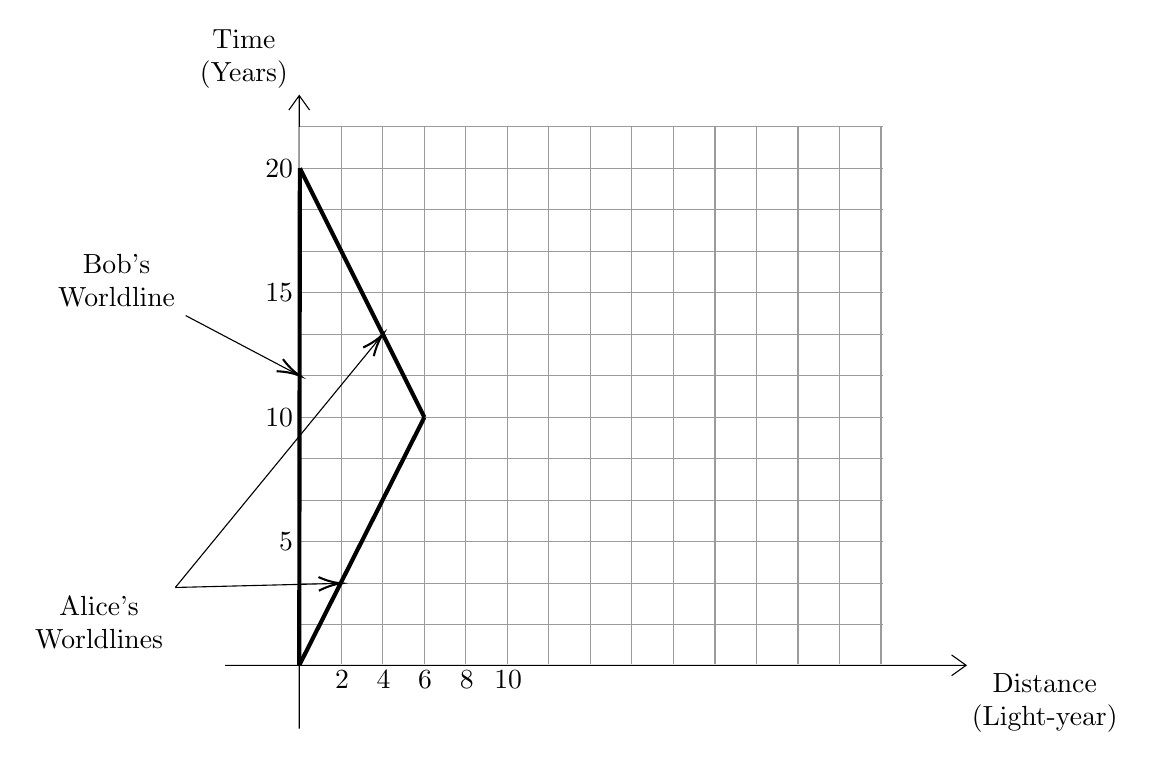
\begin{tikzpicture}[x=0.75pt,y=0.75pt,yscale=-1,xscale=1]
%uncomment if require: \path (0,420); %set diagram left start at 0, and has height of 420

%Shape: Axis 2D [id:dp05573369305563469] 
\draw  (164,323.5) -- (521,323.5)(199.7,49) -- (199.7,354) (514,318.5) -- (521,323.5) -- (514,328.5) (194.7,56) -- (199.7,49) -- (204.7,56)  ;
%Shape: Grid [id:dp24983811424563274] 
\draw  [draw opacity=0] (200,64) -- (481,64) -- (481,323) -- (200,323) -- cycle ; \draw  [color={rgb, 255:red, 155; green, 155; blue, 155 }  ,draw opacity=1 ] (200,64) -- (200,323)(220,64) -- (220,323)(240,64) -- (240,323)(260,64) -- (260,323)(280,64) -- (280,323)(300,64) -- (300,323)(320,64) -- (320,323)(340,64) -- (340,323)(360,64) -- (360,323)(380,64) -- (380,323)(400,64) -- (400,323)(420,64) -- (420,323)(440,64) -- (440,323)(460,64) -- (460,323)(480,64) -- (480,323) ; \draw  [color={rgb, 255:red, 155; green, 155; blue, 155 }  ,draw opacity=1 ] (200,64) -- (481,64)(200,84) -- (481,84)(200,104) -- (481,104)(200,124) -- (481,124)(200,144) -- (481,144)(200,164) -- (481,164)(200,184) -- (481,184)(200,204) -- (481,204)(200,224) -- (481,224)(200,244) -- (481,244)(200,264) -- (481,264)(200,284) -- (481,284)(200,304) -- (481,304) ; \draw  [color={rgb, 255:red, 155; green, 155; blue, 155 }  ,draw opacity=1 ]  ;
%Straight Lines [id:da8614004001055997] 
\draw [line width=1.5]    (199.7,323.5) -- (260,204) ;
%Straight Lines [id:da31958266480703523] 
\draw [line width=1.5]    (200,84) -- (260,204) ;
%Straight Lines [id:da118241818687711] 
\draw [line width=1.5]    (200,84) -- (199.7,323.5) ;
%Straight Lines [id:da8500340120601242] 
\draw    (145,155) -- (198.23,183.07) ;
\draw [shift={(200,184)}, rotate = 207.8] [color={rgb, 255:red, 0; green, 0; blue, 0 }  ][line width=0.75]    (10.93,-3.29) .. controls (6.95,-1.4) and (3.31,-0.3) .. (0,0) .. controls (3.31,0.3) and (6.95,1.4) .. (10.93,3.29)   ;
%Straight Lines [id:da8248865101372049] 
\draw    (140,286) -- (238.73,165.55) ;
\draw [shift={(240,164)}, rotate = 129.34] [color={rgb, 255:red, 0; green, 0; blue, 0 }  ][line width=0.75]    (10.93,-3.29) .. controls (6.95,-1.4) and (3.31,-0.3) .. (0,0) .. controls (3.31,0.3) and (6.95,1.4) .. (10.93,3.29)   ;
%Straight Lines [id:da5391136210716794] 
\draw    (140,286) -- (218,284.05) ;
\draw [shift={(220,284)}, rotate = 178.57] [color={rgb, 255:red, 0; green, 0; blue, 0 }  ][line width=0.75]    (10.93,-3.29) .. controls (6.95,-1.4) and (3.31,-0.3) .. (0,0) .. controls (3.31,0.3) and (6.95,1.4) .. (10.93,3.29)   ;

% Text Node
\draw (197.81,47) node [anchor=south east] [inner sep=0.75pt]   [align=left] {\begin{minipage}[lt]{35.23pt}\setlength\topsep{0pt}
\begin{center}
Time\\(Years)
\end{center}

\end{minipage}};
% Text Node
\draw (521,326) node [anchor=north west][inner sep=0.75pt]   [align=left] {\begin{minipage}[lt]{54.88pt}\setlength\topsep{0pt}
\begin{center}
Distance\\(Light-year)
\end{center}

\end{minipage}};
% Text Node
\draw (198,264) node [anchor=east] [inner sep=0.75pt]   [align=left] {5};
% Text Node
\draw (198,204) node [anchor=east] [inner sep=0.75pt]   [align=left] {10};
% Text Node
\draw (198,144) node [anchor=east] [inner sep=0.75pt]   [align=left] {15};
% Text Node
\draw (198,84) node [anchor=east] [inner sep=0.75pt]   [align=left] {20};
% Text Node
\draw (220.38,325) node [anchor=north] [inner sep=0.75pt]   [align=left] {2};
% Text Node
\draw (240.38,325) node [anchor=north] [inner sep=0.75pt]   [align=left] {4};
% Text Node
\draw (260.38,325) node [anchor=north] [inner sep=0.75pt]   [align=left] {6};
% Text Node
\draw (280.38,325) node [anchor=north] [inner sep=0.75pt]   [align=left] {8};
% Text Node
\draw (300.38,325) node [anchor=north] [inner sep=0.75pt]   [align=left] {10};
% Text Node
\draw (143,152) node [anchor=south east] [inner sep=0.75pt]   [align=left] {\begin{minipage}[lt]{45.05pt}\setlength\topsep{0pt}
\begin{center}
Bob's\\Worldline
\end{center}

\end{minipage}};
% Text Node
\draw (138,289) node [anchor=north east] [inner sep=0.75pt]   [align=left] {\begin{minipage}[lt]{50.15pt}\setlength\topsep{0pt}
\begin{center}
Alice's\\Worldlines
\end{center}

\end{minipage}};


\end{tikzpicture}

          \caption{Bob and Alice's Spacetime Diagrams}
          \label{fig:5}
        \end{figure}

      \item Bob's worldline is vertical, signifying no motion

      \item Alice has two straight lines (two inertial reference frames), as she moves to and then away from the distance object

      \item Light signals travel from Bob to Alice along the $45^{\circ}$ direction

      \item Light signals travel from Alice to bob along the $-45^{\circ}$ direction

    \end{itemize}

  \item Lorentz transformation prevents relative speed from reaching or exceeding $c$

    \section{Relativistic Dynamics}

  \item Applies to the energies and momentums of objects

    \newpage

    \begin{figure}[h!]
      \centering
      \tikzset{every picture/.style={line width=0.75pt}} %set default line width to 0.75pt        

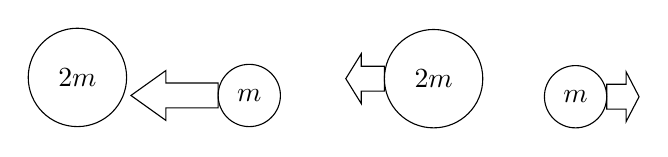
\begin{tikzpicture}[x=0.75pt,y=0.75pt,yscale=-.6,xscale=.6]
%uncomment if require: \path (0,420); %set diagram left start at 0, and has height of 420

%Shape: Circle [id:dp17026976972223973] 
\draw   (98,116.5) .. controls (98,94.68) and (115.68,77) .. (137.5,77) .. controls (159.32,77) and (177,94.68) .. (177,116.5) .. controls (177,138.32) and (159.32,156) .. (137.5,156) .. controls (115.68,156) and (98,138.32) .. (98,116.5) -- cycle ;
%Shape: Circle [id:dp1732786352755724] 
\draw   (250.5,131) .. controls (250.5,117.19) and (261.69,106) .. (275.5,106) .. controls (289.31,106) and (300.5,117.19) .. (300.5,131) .. controls (300.5,144.81) and (289.31,156) .. (275.5,156) .. controls (261.69,156) and (250.5,144.81) .. (250.5,131) -- cycle ;
%Left Arrow [id:dp2694928798272458] 
\draw   (180.5,131) -- (208.5,111) -- (208.5,121) -- (250.5,121) -- (250.5,141) -- (208.5,141) -- (208.5,151) -- cycle ;
%Shape: Circle [id:dp29195586713142996] 
\draw   (384,117.5) .. controls (384,95.68) and (401.68,78) .. (423.5,78) .. controls (445.32,78) and (463,95.68) .. (463,117.5) .. controls (463,139.32) and (445.32,157) .. (423.5,157) .. controls (401.68,157) and (384,139.32) .. (384,117.5) -- cycle ;
%Shape: Circle [id:dp47955008763043105] 
\draw   (512.5,132) .. controls (512.5,118.19) and (523.69,107) .. (537.5,107) .. controls (551.31,107) and (562.5,118.19) .. (562.5,132) .. controls (562.5,145.81) and (551.31,157) .. (537.5,157) .. controls (523.69,157) and (512.5,145.81) .. (512.5,132) -- cycle ;
%Left Arrow [id:dp529662098694889] 
\draw   (353,117.5) -- (365.4,97.5) -- (365.4,107.5) -- (384,107.5) -- (384,127.5) -- (365.4,127.5) -- (365.4,137.5) -- cycle ;
%Right Arrow [id:dp8432969383145832] 
\draw   (562.5,122) -- (578.1,122) -- (578.1,112) -- (588.5,132) -- (578.1,152) -- (578.1,142) -- (562.5,142) -- cycle ;

% Text Node
\draw (137.5,116.5) node   [align=left] {$\displaystyle 2m$};
% Text Node
\draw (275.5,131) node   [align=left] {$\displaystyle m$};
% Text Node
\draw (423.5,117.5) node   [align=left] {$\displaystyle 2m$};
% Text Node
\draw (537.5,132) node   [align=left] {$\displaystyle m$};


\end{tikzpicture}

      \caption{Momentum Collision}
      \label{fig:6}
    \end{figure}

  \item Assuming the $2m$ mass is initially at rest, and $m$ is moving at $-.75c$, how would the final result be derived?

  \item Using conservation of momentum, there should be $-.75mc$ total momentum at the end; however, a Lorentz transformation must be used when working with relativistic dynamics
    
  \item So is momentum conserved in relativistic dynamics?

    \begin{itemize}

      \item No, $p_i \neq p_f$

    \end{itemize}

  \item Thus, it was necessary to modify the mass in relativistic dynamics so that conservation of momentum holds true

    \begin{itemize}

      \item The new mass had to be a function of the velocity

      \item The following function was hypothesized, with $v$ as the speed of an object in an inertial reference frame:

        $$\boxed{m(v)=\frac{m}{\sqrt{1-\dfrac{v^2}{c^2}}}}$$

      \item At $v=0$, the mass would be as normal, also known as the rest mass

      \item But, as $v$ approaches $c$, the mass approaches infinity!

      \item This would mean relativistic momentum is defined as:

        $$\overline{p}=m(v)\overline{v}\Rightarrow \frac{1}{\sqrt{1-\dfrac{v^2}{c^2}}}m\overline{v}$$

      \item The relativistic momentum conservation formula can then be applied to relativistic kinetic energy conservation

    \end{itemize}

  \item Kinetic Energy in Relativity Theory

    \begin{itemize}

      \item In classical physics, the work-energy theorem is:

        $$K=W=\int_0^x F\,dx\Rightarrow F=\frac{d\overline{p}}{dt}\Rightarrow \int_0^{\overline{p}} \frac{dx}{dt}\,dp$$

      \item $\dfrac{dx}{dt}=v$, so we have velocity involved

      \item Substituting and using integration by parts, we get:

        $$\int_0^p v\,dp=pv-\int p\,dv$$

      \item This means that the kinetic energy may be defined as:

        $$K=pv-\int_0^v p\,dv$$

        $$K=\frac{mv^2}{\sqrt{1-\dfrac{v^2}{c^2}}}-\int_0^v \frac{mv}{\sqrt{1-\dfrac{v^2}{c^2}}}\,dv$$

        $$K=\frac{mv^2}{\sqrt{1-\dfrac{v^2}{c^2}}}+mc^2\sqrt{1-\dfrac{v^2}{c^2}}-mc^2$$

        $$\boxed{K=\frac{mc^2}{\sqrt{1-\dfrac{v^2}{c^2}}}-mc^2}$$

      \item Sometimes, this formula is simplified as $K=\gamma mc^2-mc^2$

        \begin{itemize}

          \item $\gamma mc^2$ is referred to as the relativistic total energy ($E$)

          \item $mc^2$ is referred to as the rest energy ($E_0$)

            $$E=K+E_0=\gamma mc^2$$

        \end{itemize}

      \item This is the relativistic kinetic energy

      \item When $v$ approaches $c$, kinetic energy approaches $\infinity$

      \item This means it will take infinite energy to accelerate to the speed of light

    \end{itemize}

  \item Bertozz et al Experiment (1964)

    \begin{itemize}

      \item Accelerated an electron using an electric field

      \item Found that electrons could not be accelerated to the speed of light

      \item Verified the relativistic energy theorem

    \end{itemize}

  \item The Energy-Momentum Relationship can be defined as:

    $$E^2=(mc^2)^2+(pc)^2$$

    \begin{itemize}

      \item When $v\approx c$, $E\approx pc$

      \item This means, for massless particles (\textit{e}.\textit{g}. photons)

        $$\boxed{E=pc}$$

    \end{itemize}

\end{itemize}

\end{document}

